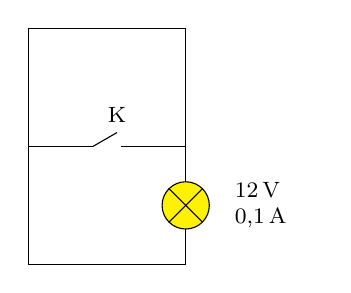
\begin{tikzpicture}[
	font=\footnotesize,
	]
	\draw (0,0)rectangle(2,3);
	\draw (0,1.5)--++(2,0);
	\pileL{shift={(0,.75)}}{4,5\,V};
	\voltmetre{shift={(1,3)}};
	\draw[fill=yellow,shift={(2,0.75)}]circle(.3);
	\draw[shift={(2,0.75)}](45:.3)--(-135:.3);
	\draw[shift={(2,0.75)}](135:.3)--(-45:.3);
	\fill[white,shift={(1,1.5)}](-5pt,-5pt)rectangle(5pt,5pt);
	\draw[black,shift={(1,1.5)}](-5pt,0)--++(30:10pt)node[above]{K};
	\draw (2.5,.75)node[right,text width=1cm]{12\,V 0,1\,A};
\end{tikzpicture}